\documentclass[border=6pt]{standalone}
\usepackage{tikz}
\usetikzlibrary{arrows.meta, positioning, calc, fit, backgrounds}
\usepackage{xcolor}
\usepackage{amsmath}

% Brand colors
\definecolor{Garnet}{HTML}{73000A}
\definecolor{Atlantic}{HTML}{466A9F}
\definecolor{Congaree}{HTML}{1F414D}
\definecolor{Horseshoe}{HTML}{65780B}
\definecolor{Rose}{HTML}{CC2E40}
\definecolor{LightGray}{HTML}{ECECEC}
\definecolor{Black90}{HTML}{363636}
\definecolor{WarmGrey}{HTML}{676156}

\begin{document}
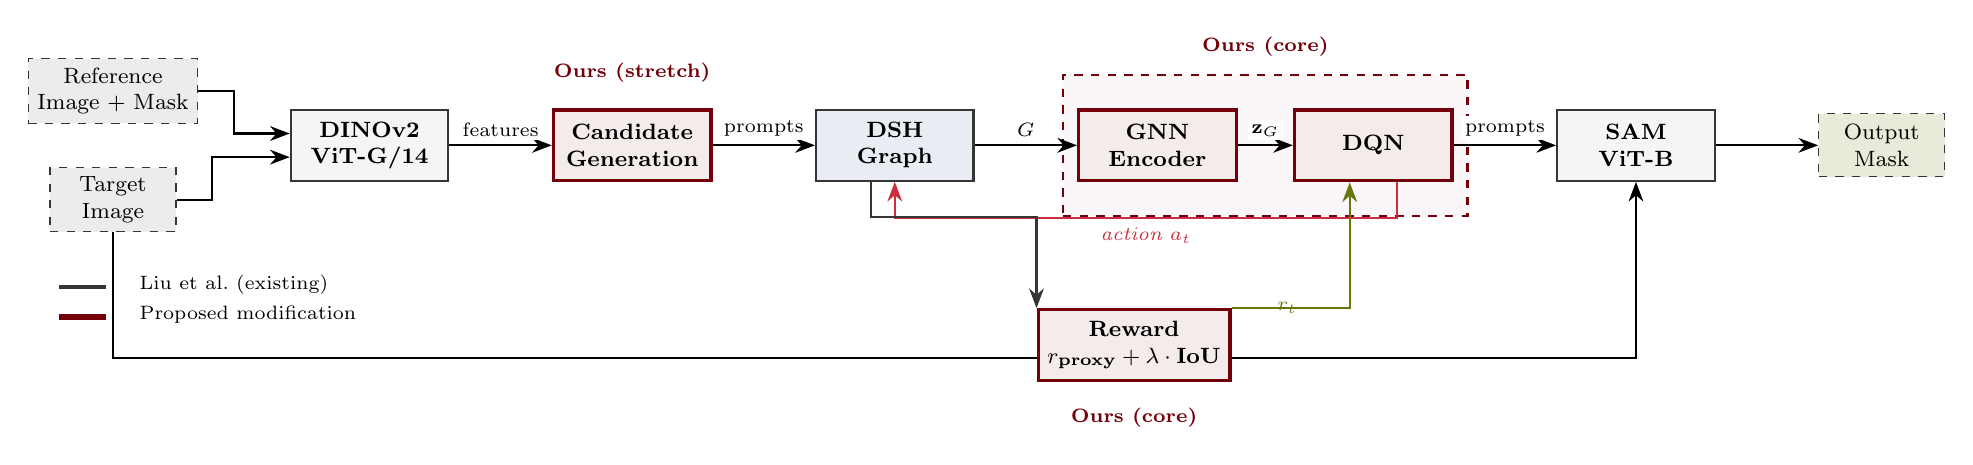
\begin{tikzpicture}[
    model/.style={
        draw=Black90, thick, minimum width=2.0cm, minimum height=0.9cm,
        align=center, font=\footnotesize\bfseries
    },
    data/.style={
        draw=Black90, dashed, minimum width=1.6cm, minimum height=0.8cm,
        align=center, font=\footnotesize
    },
    ours/.style={
        draw=Garnet, very thick, minimum width=2.0cm, minimum height=0.9cm,
        align=center, font=\footnotesize\bfseries
    },
    arr/.style={-{Stealth[length=2.5mm]}, thick},
    lbl/.style={font=\scriptsize, fill=white, inner sep=1.5pt},
    ourlbl/.style={font=\scriptsize\bfseries, text=Garnet},
    every node/.style={font=\footnotesize}
]

% =============================================
% ROW 1: Inputs (stacked vertically)
% =============================================
\node[data, fill=LightGray] (ref) {Reference\\Image + Mask};
\node[data, fill=LightGray, below=0.55cm of ref] (tgt) {Target\\Image};

% =============================================
% DINO feature extraction
% =============================================
\node[model, fill=LightGray!50, right=1.3cm of $(ref.east)!0.5!(tgt.east)$] (dino) {DINOv2\\ViT-G/14};

\draw[arr] (ref.east) -- ++(0.45,0) |- ([yshift=0.15cm]dino.west);
\draw[arr] (tgt.east) -- ++(0.45,0) |- ([yshift=-0.15cm]dino.west);

% =============================================
% Candidate generation (stretch goal)
% =============================================
\node[ours, fill=Garnet!8, right=1.3cm of dino] (cand) {Candidate\\Generation};

\draw[arr] (dino.east) -- (cand.west)
    node[lbl, midway, above=0.05cm] {features};

\node[ourlbl, above=0.2cm of cand] {Ours (stretch)};

% =============================================
% DSH Graph
% =============================================
\node[model, fill=Atlantic!12, right=1.3cm of cand] (graph) {DSH\\Graph};

\draw[arr] (cand.east) -- (graph.west)
    node[lbl, midway, above=0.05cm] {prompts};

% =============================================
% GNN + DQN (replaces Q-table)
% =============================================
\node[ours, fill=Garnet!8, right=1.3cm of graph] (gnn) {GNN\\Encoder};
\node[ours, fill=Garnet!8, right=0.7cm of gnn] (dqn) {DQN};

\draw[arr] (graph.east) -- (gnn.west)
    node[lbl, midway, above=0.05cm] {$G$};
\draw[arr] (gnn.east) -- (dqn.west)
    node[lbl, midway, above=0.05cm] {$\mathbf{z}_G$};

% Dashed box around GNN + DQN
\begin{scope}[on background layer]
    \node[draw=Garnet, dashed, thick, fill=Garnet!3,
          inner xsep=5pt, inner ysep=12pt,
          fit=(gnn)(dqn)] (gnnbox) {};
\end{scope}
\node[ourlbl, above=0.1cm of gnnbox] {Ours (core)};

% =============================================
% SAM
% =============================================
\node[model, fill=LightGray!50, right=1.3cm of dqn] (sam) {SAM\\ViT-B};

\draw[arr] (dqn.east) -- (sam.west)
    node[lbl, midway, above=0.05cm] {prompts};

% Target image to SAM (clean route along bottom)
\draw[arr] (tgt.south) -- ++(0,-1.6) -| (sam.south);

% =============================================
% Output
% =============================================
\node[data, fill=Horseshoe!15, right=1.3cm of sam] (mask) {Output\\Mask};

\draw[arr] (sam.east) -- (mask.west);

% =============================================
% RL loop: DQN action -> Graph, Graph state -> Reward, Reward -> DQN
% =============================================

% Reward box centered below graph--dqn span
\node[ours, fill=Garnet!8, minimum width=2.4cm,
      below=1.6cm of $(graph.south)!0.5!(dqn.south)$] (reward)
    {Reward\\$r_{\text{proxy}} + \lambda \cdot \text{IoU}$};

\node[ourlbl, below=0.2cm of reward] {Ours (core)};

% DQN -> action -> Graph (loop above the reward, below the main row)
\draw[arr, Rose] ([xshift=0.3cm]dqn.south) -- ++(0,-0.45) -| (graph.south)
    node[pos=0.25, below, font=\scriptsize\itshape, text=Rose] {action $a_t$};

% Graph -> Reward (state feeds down)
\draw[arr, Black90] ([xshift=-0.3cm]graph.south) -- ++(0,-0.45) -| (reward.north west)
    node[pos=0.0, left, font=\scriptsize] {};

% Reward -> DQN (reward signal back up)
\draw[arr, Horseshoe] (reward.north east) -| ([xshift=-0.3cm]dqn.south)
    node[pos=0.15, right, font=\scriptsize, text=Horseshoe] {$r_t$};

% =============================================
% Legend (bottom-left, below everything)
% =============================================
\node[anchor=north west, font=\scriptsize] at ([yshift=-0.4cm]tgt.south west) {
    \begin{tabular}{@{}cl@{}}
    \textcolor{Black90}{\rule{0.6cm}{1.5pt}} & Liu et al.~(existing) \\[3pt]
    \textcolor{Garnet}{\rule{0.6cm}{2pt}} & Proposed modification \\
    \end{tabular}
};

\end{tikzpicture}
\end{document}
